\chapter{The Sensory Afferent Database}\label{ch:database}
\graphicspath{{../Figures/50-database/}{figs/50-database/}}

Choosing a sensory connection for a locomotor controller requires more than the name of a receptor. A researcher needs to know which nerve was stimulated, which motor neurons responded, and whether the animal was at rest or moving. Those details are scattered across studies that used different species, preparations, and tasks. I developed the Sensory Afferent Database (SADb) to keep a proposed feedback pathway linked to the experiment that supports it. The collection also links to computational models so that a researcher can compare an experimental finding with the assumptions used to represent it. This work forms part of the AARL's NeuroNex Communication, Coordination, and Control in Nervous Systems (C3NS) effort.

\noindent Presentation credits: The SADb resource was presented as an abstract and poster at Neuroscience 2023 \citep{bolen_sensory_2023}. The AI-assisted curation study was presented as an abstract and poster at Neuroscience 2024 \citep{bolen_using_2024}.

\begin{samepage}
Open SADb Explorer in a browser using \path{SADb_audit/app/sadb_app.html} in the project repository. Three tabs work offline (Figure~\ref{fig:sadb_clusters}A). Table retrieves individual records, Pivot counts papers that share classifications, and Bubble map follows citations. Search (online) queries the OpenAlex bibliographic index for candidates to save for later curation.\par
\end{samepage}

\begin{sidewaysfigure}[p]
\centering
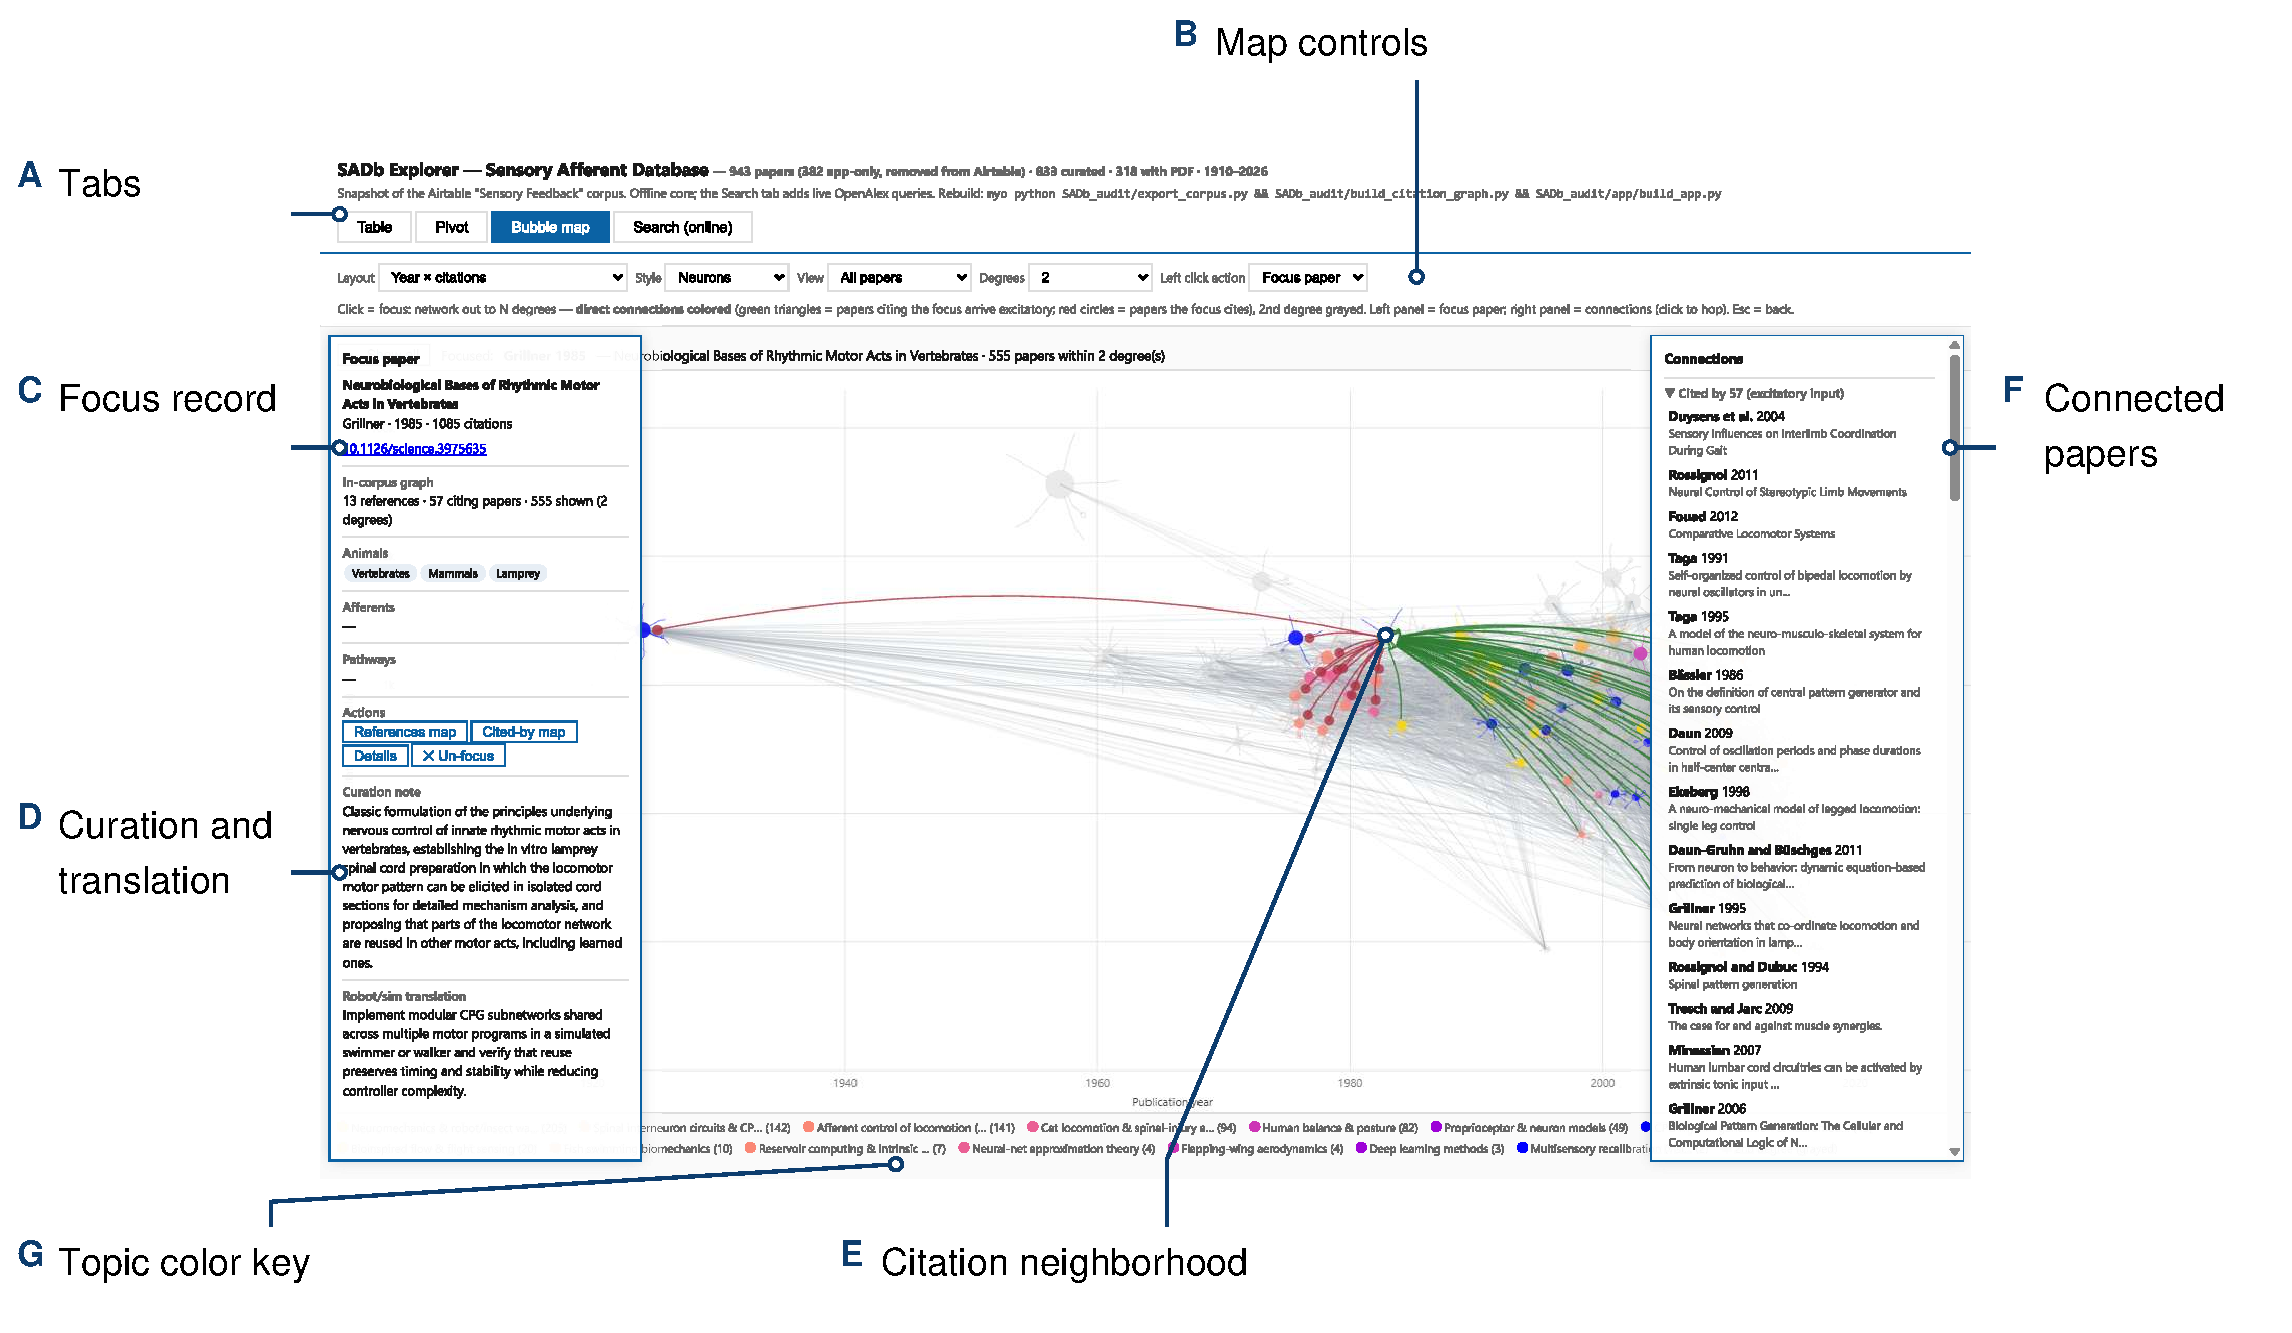
\includegraphics[width=\linewidth]{sadb_bubble.pdf}
\caption[SADb Explorer citation-map functions]{Citation map of the 943 Papers in an earlier Explorer snapshot, with Grillner (1985) selected. Callouts identify the four main tabs \textbf{(A)}, map controls \textbf{(B)}, selected record \textbf{(C)}, curation and translation notes \textbf{(D)}, citation neighborhood \textbf{(E)}, connected papers \textbf{(F)}, and the topic-cluster color key \textbf{(G)}.}
\label{fig:sadb_clusters}
\end{sidewaysfigure}

\begin{samepage}
I curated the database in Airtable, an online database system. Linked tables connect papers, pathways, and models. Exporting the records with those links preserves the route from a pathway name to the relevant paper, its curation note, and the original study in the standalone Explorer.\par
\end{samepage}

\section{Curation Methods}\label{sec:sadb_methods}

SADb is a curated research collection, rather than a registered systematic review or an exhaustive search of every relevant publication. I first collected records from selected AARL and personal Zotero collections used for previous papers on locomotion and postural balance, together with a few records already curated in Airtable by my advisor, Dr. Hunt. Duplicate Zotero entries describing the same publication were combined into a single record using DOI and title matching. I expanded the collection through keyword searches, references cited by relevant papers, and searches for subsequent papers citing them.

I initially imported the broader Zotero collections as groups, then narrowed the working base to sensory feedback in locomotion and posture. I retained records reporting sensory-afferent measurements, investigating feedback in locomotion or posture, or modeling a relevant sensory pathway. I removed records outside this scope from the working base. I also flagged records whose source text I could not locate, including conference posters found through ResearchRabbit, and removed them from that base. The application preserves the broader collection as archived records, which users can distinguish with the archive filter. Figure~\ref{fig:sadb_curation_workflow} summarizes the curation sequence. For retained papers, I recorded the animal or human study context where applicable, afferent class, feedback pathway, and the mechanism described by the study.

I implemented a monthly literature watch that queries OpenAlex and Crossref for candidate additions matching selected authors and keywords. Its search terms include ``Ia afferent,'' ``Ib afferent,'' ``muscle spindle,'' ``proprioceptive feedback,'' and ``central pattern generator.'' The script removes DOI and version duplicates, verifies shortlisted DOIs through Crossref, and writes a shortlist for manual curation. Source-access limitations are recorded with the shortlist; inclusion and classification decisions remain manual.

\begin{figure}[htbp]
\centering
\usetikzlibrary{arrows.meta}
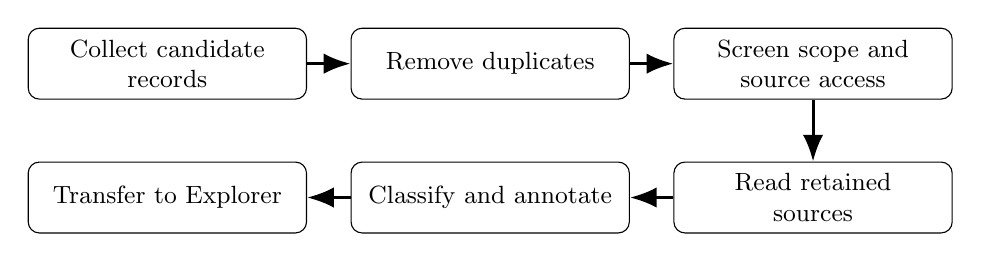
\begin{tikzpicture}[every node/.style={font=\small},curationstep/.style={draw,rounded corners,align=center,text width=3.3cm,minimum height=0.9cm},flow/.style={-{Latex[length=3.4mm,width=2.6mm]},line width=1.1pt}]
\node[curationstep] (a) at (0,0) {\mbox{Collect candidate}\\records};
\node[curationstep] (b) at (4.1,0) {Remove duplicates};
\node[curationstep] (c) at (8.2,0) {Screen scope and source access};
\node[curationstep] (d) at (8.2,-1.7) {\mbox{Read retained}\\sources};
\node[curationstep] (e) at (4.1,-1.7) {Classify and annotate};
\node[curationstep] (f) at (0,-1.7) {Transfer to Explorer};
\draw[flow] (a)--(b);\draw[flow] (b)--(c);\draw[flow] (c)--(d);\draw[flow] (d)--(e);\draw[flow] (e)--(f);
\end{tikzpicture}
\caption{Curation of SADb records. The monthly search supplies candidate papers. A curator reads each source, decides whether it belongs in the collection, and records the classifications and supporting evidence.}
\label{fig:sadb_curation_workflow}
\end{figure}

\section{Results: Application and Corpus Coverage}\label{sec:sadb_corpus}

The searchable Table contains 1,393 entries. These comprise 943 Papers, 247 Models, 157 Review Papers, 42 Feedback pathways, and 4 Recorders. It includes archived entries. Pivot and Bubble map draw from the 943 Papers. Appendix~\ref{app:sadb_records} explains which records were retained in the working database and how to interpret the coverage counts.

Within the application's Papers category, containing 943 entries, 833 carry curation notes, 606 have tags for the animals or human participants studied, 316 carry animal-study assessments, 119 link to feedback pathways, 95 carry an afferent classification, and 363 carry robot-or-simulation translation notes. DOI identifiers are present for 892 papers, and 318 have attached-PDF indicators. Of these Papers, 730 cite at least one other Paper in the collection. Counting both citing and cited papers gives 816 distinct Papers connected by 11,130 directed citation pairs. The Louvain algorithm identifies groups of papers with relatively dense citation links. The application labels these communities as 18 named topic clusters (Figure~\ref{fig:sadb_clusters}, callout~(G)), which help users navigate related studies in the Bubble map tab.

The Table tab retrieves both a paper and the evidence recorded for it. For example, choosing \emph{Ib disynaptic excitation} in the \emph{Pathway} filter returns six Papers (Figure~\ref{fig:sadb_explorer}). Select the row for \citet{mccrea_disynaptic_1995} to open its record. The drawer shows the source DOI, the Cat classification, both Ia and Ib afferent tags, and two pathway labels, \emph{Ib disynaptic excitation} and \emph{Ib disynaptic inhibition}. Reading the experiment explains why both labels apply.

\begin{figure}[H]
\centering
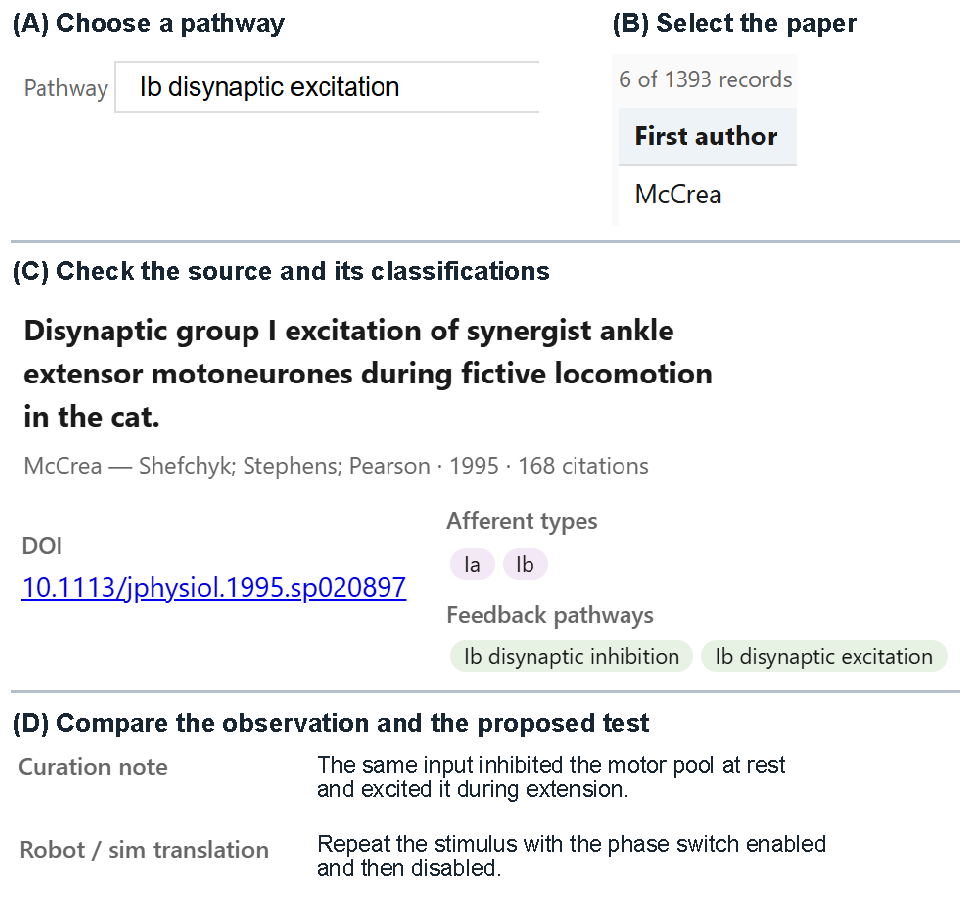
\includegraphics[width=\textwidth]{sadb_table_record_guide.pdf}

\caption[Finding the experimental evidence for a pathway]{The SADb Explorer pathway filter \textbf{(A)} returns six Papers. Selecting the McCrea row in the results \textbf{(B)} opens the record \textbf{(C)}, which gives the source DOI, the afferent classes, and the two pathway labels. The DOI opens the experiment that supports the classifications.}
\label{fig:sadb_explorer}
\end{figure}

\subsection{From a Pathway Record to a Controller Rule}\label{sec:sadb_worked_rule}
In decerebrate cats at rest, stimulating the plantaris nerve at group~I strength inhibited medial gastrocnemius motor neurons. With the same stimulus during extension in midbrain-evoked fictive locomotion, the recorded response was excitatory. In this preparation the neural rhythm was present while the animal was immobilized. Nerve stimulation recruited group~I fibers and did not isolate Ib fibers.

Figure~\ref{fig:sadb_group_i_rule} shows one rule a modeler could take from this record. During simulated rest, a brief input from the plantaris group~I pathway would reduce activity in the synergist motor pool. During the active extensor phase, the same input would increase its activity. The measurements constrain the sign and timing of the net response. Choosing the interneurons, synaptic strengths, and delays that produce it is a separate modeling decision. Appendix~\ref{app:sadb_records} shows how the result changes in a different preparation.

\begin{figure}[!htbp]
\centering
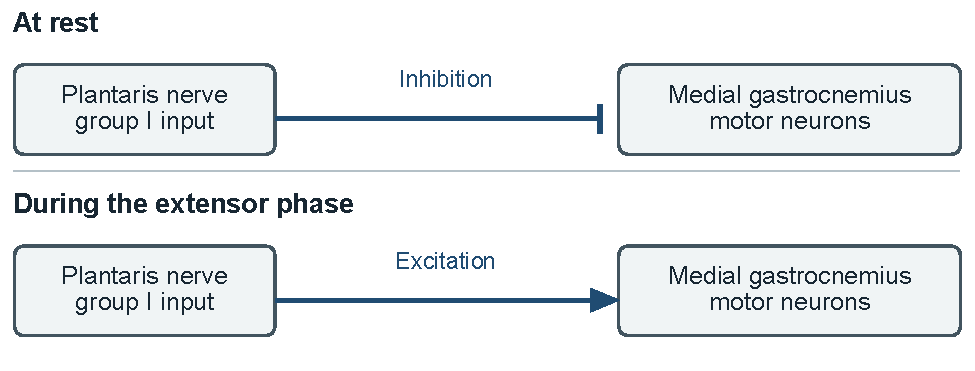
\includegraphics[width=\textwidth]{sadb_group_i_rule.pdf}
\caption[An experimental constraint on a sensory feedback rule]{The plantaris nerve stimulus and recorded medial gastrocnemius motor pool were the same in both conditions. Stimulation inhibited the motor neurons at rest and excited them during the extensor phase of midbrain-evoked fictive locomotion \citep{mccrea_disynaptic_1995}. The two signed connections represent a candidate model's net response through spinal circuitry.}
\label{fig:sadb_group_i_rule}
\end{figure}
\FloatBarrier

\subsection{Comparing Groups of Papers}

Pivot answers a different question. With the Table filters cleared, choose \emph{Afferent types} and \emph{Animal}, then select the Ib--Cat cell (Figure~\ref{fig:sadb_pivot}). Table opens the 21 Papers counted in that cell. \emph{Back to pivot} restores the comparison. A paper can carry more than one afferent or animal tag and appear in several cells. A cell count consequently describes how much material a researcher can inspect for a particular combination.

\begin{figure}[H]
\centering
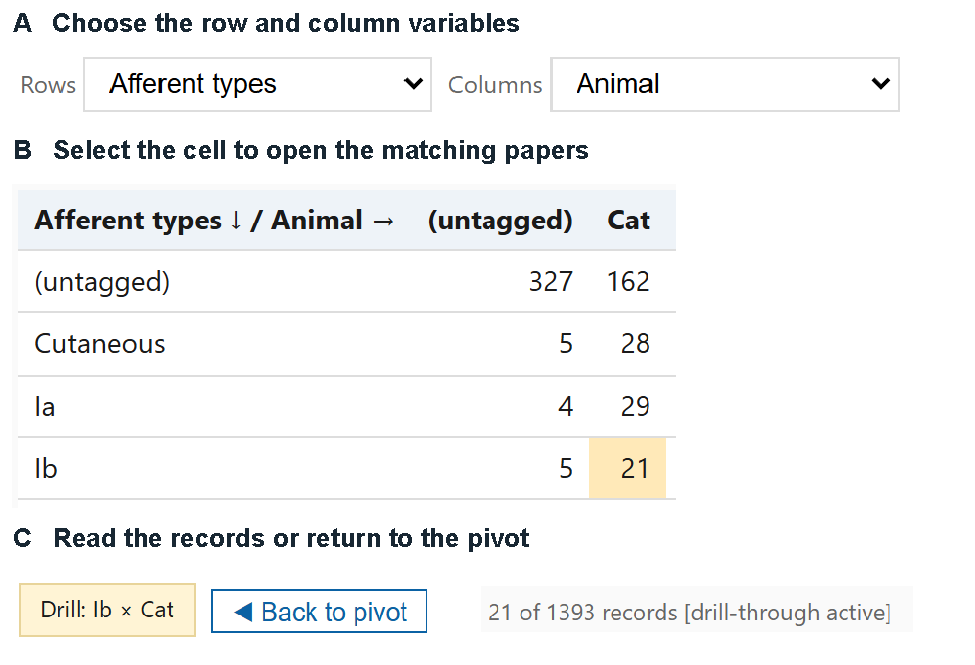
\includegraphics[width=\textwidth]{sadb_pivot_guide.pdf}
\caption[The SADb Explorer pivot view]{With afferent type and animal selected \textbf{(A)}, the Ib row and Cat column intersect at 21 \textbf{(B)}. Selecting the cell opens the 21 matching Papers in Table. The return control restores the pivot \textbf{(C)}.}
\label{fig:sadb_pivot}
\end{figure}

\subsection{Following Citations in Bubble Map}

The Bubble map tab offers two selectable layouts (Figure~\ref{fig:sadb_clusters}). The year--citations layout places publication year on the horizontal axis and citation count on a logarithmic vertical axis. The topic landscape instead draws papers as nodes joined by citation links. A spring-layout algorithm balances attraction along links with repulsion between nodes to arrange connected groups together. Its coordinates arrange the network; neither axis measures publication year or citation count. The user controls the layout, display style, record grouping, citation-neighborhood depth, and click action (Figure~\ref{fig:sadb_clusters}, callout~(B)).

Selecting a paper makes it the reference for the displayed citation neighborhood; the application calls this the focus paper. Its source information appears in the left record area (Figure~\ref{fig:sadb_clusters}, callout~(C)), together with its curation note and notes on possible applications to a robot or simulation (Figure~\ref{fig:sadb_clusters}, callout~(D)). The neighborhood selector in callout~(B) displays papers up to one, two, or three citation links from the focus paper. Callout~(E) marks the resulting neighborhood, which includes both references and citing papers. A two-link neighborhood adds one level beyond the directly connected papers. Directly connected papers retain color, while papers reached through additional links are gray. In the illustrated neighborhood of the Grillner (1985) focus paper, 57 in-corpus papers cite it, it cites 13 in-corpus papers, and the two-link display contains 555 papers including the focus paper itself. Green triangles identify papers that cite the focus paper, and red circles identify papers cited by it.

The connection list separates papers citing the focus paper from its references (Figure~\ref{fig:sadb_clusters}, callout~(F)). Selecting a listed paper makes it the new focus paper, allowing a reader to follow the development of an idea without repeatedly searching for individual titles. The reference-only and cited-by views isolate either direction, and the detail action opens the underlying record. A researcher can therefore start from a known experiment, inspect earlier studies supporting it, follow subsequent models or experiments citing it, and read the associated translation notes before choosing a candidate pathway for simulation.

\begingroup

The feedback-pathway records extend beyond the mammalian core of Table~\ref{tab:sadb_pathways}: paired excitation and inhibition records cover the chordotonal organs and trochanteral hair plates of insect legs, a load-feedback record covers the campaniform sensilla, and further records hold fictive locomotion without sensory feedback (12 linked papers), group III/IV fatigue, and one paper each for somatosensory, vestibular, and visual contributions to postural control. These records let a researcher identify candidate pathways across species. Chapter~\ref{ch:sns} tests selected mammalian feedback connections in specific controllers.
\par
\endgroup

\subsection{AI-Assisted Literature Triage}\label{sec:sadb_triage}

I evaluated AI-assisted literature identification, summarization, and categorization, judging the outputs against how well and how quickly I could complete these tasks myself. This work was presented at Neuroscience 2024 \citep{bolen_using_2024}. The comparison includes ResearchRabbit, Litmaps, txyz, SciSpace, and MirrorThink. Some tools helped identify related papers or summarize straightforward material, but categorization remained inadequate: none received a good rating, and only txyz was rated adequate. Complex models and nuanced physiological findings required substantial human correction. The tools therefore offered limited help with the central task of accurately assigning papers to database categories. I made the final inclusion, classification, and removal decisions.

\section{Discussion}
\subsection{Uses of the Database}\label{sec:sadb_use}

For a modeler, the value of a curated record lies in the distinctions it preserves. The plantaris experiment yielded a different sign at rest and during extension. A controller with a single positive gain for every group~I input would miss that difference. A modeler can return to the source to choose which preparation the controller should represent and what stimulus would test it.

Table~\ref{tab:sadb_afferents} in Appendix~\ref{app:sadb_records} relates each receptor to a possible model input. Table~\ref{tab:sadb_pathways} lists the pathway records and the papers linked to them. For example, \emph{Ia monosynaptic excitation} concerns the motor pool of the muscle containing the spindle, while \emph{Ia reciprocal inhibition} concerns the antagonist motor pool and an intervening inhibitory neuron. Selecting the pathway as well as the afferent specifies which connection the researcher wants to examine.

SADb supplies records and source connections through which a researcher can compare experimental evidence with model assumptions. \citet{ting_limited_2005} linked muscle-activation synergies to limb endpoint-force vectors in cats responding to support-surface translations. \citet{latash_organization_2020} compared cat stepping patterns with a mathematical model to investigate how rhythm-generator operation could change with control drive under tied-belt and split-belt conditions. The first study connects measured muscle activity to postural output; the second tests a candidate circuit explanation for locomotor phase patterns. Following the source papers exposes these differences in task, preparation, and explanation.

Comparing model records helps a researcher identify how sensory afferent pathways depend on the mechanical model and task. \citet{geyer_musclereflex_2010} generated walking in a human musculoskeletal model using phase-dependent muscle reflexes. In a rat neuromechanical model, \citet{deng_biomechanical_2022} found that biomechanical entrainment and sensory feedback reduced behavioral differences associated with alternative CPG parameter choices. Model records provide starting points for comparing these approaches and two-level rhythm-generation and pattern-formation architectures \citep{rybak_modelling_2006}. For the controllers in Chapter~\ref{ch:sns}, pathway selection is followed by explicit choices and tests of receptor dynamics, gains, delays, and species-specific assumptions.

The balance, posture, and multisensory-recalibration clusters provide entry points for the vestibular and visual extensions proposed in Section~\ref{sec:fw_senses}. Searches of existing animal studies let users compare the conditions and tasks behind a proposed feedback rule before testing it in a robotic or computational model. Reusing this evidence for model-based tests supports the aim of reducing reliance on further animal experimentation (Section~\ref{sec:bg_ethics}).

SADb supplies the source, preparation, stimulus, and measured response behind a candidate rule. The rule can then be tested by holding the mechanical model fixed, changing the sensory connection, and repeating the same stimulus. Chapter~\ref{ch:sns} develops the tools for that comparison.

